% !TeX program = LuaLaTeX
\documentclass[parskip=half]{scrartcl}

\input{../name}

\usepackage{xcolor}
\usepackage{hyperref}
\hypersetup{
    colorlinks,
    linkcolor={red!50!black},
    citecolor={blue!50!black},
    urlcolor={blue!80!black}
}

\usepackage{graphicx}
\graphicspath{ {./images/} }

\usepackage{datetime2}

% Font Stuff

\usepackage{microtype}
\usepackage{fontspec}
\usepackage{unicode-math}

% Stix fonts should be auto-installed by the TeX package manager
\setmainfont{Georgia}
\setmonofont{Source Code Pro}
\setmathfont{Stix Two Math} 

% Stylistically a good match, and licensed under the Open Font License
\setsansfont{Helvetica Neue}

\newcommand{\figref}[1]{Figure~\ref{#1}}

\begin{document}

{\LARGE \textbf{\textsf{Vulnerability Report}}}
\vspace*{1em}

\textbf{Date:} \today

\textbf{Author:} \docauthor

\textbf{Student code:} \texttt{\studentcode}

\section*{Vulnerability 1}

\textbf{Risk level.} critical

The spy agency's personnel management system is openly accessible. That is, any
entity can, without authentication, view the names, jobs, and locations of
agents, as stored in the database. Moreover, any entity can acquire the password
of the day.

\textbf{Risk.} If exploited, an adversary gains valuable knowledge about the
identities, jobs, and whereabouts of spies, which is both a privacy and national
or even international security risk (spy data). Furthermore, even if the open
access is remediated, an entity may still be able to gain access to some systems
by using the leaked password, unless credentials are rotated. The password may
provide access to further systems than the open access panel.

The attack vector is broken access control, insecure design. Namely, an attacker
requires no tools or special action to gain access to the admin panel. It
suffices for an attacker to simply visit the admin panel's public URL.

Potentially applicable OWASP categories are:
\begin{enumerate}
  \item \texttt{A01:2021} -- Broken Access Control%\footnote{\url{https://owasp.org/Top10/A01_2021-Broken_Access_Control/}}
  \item \texttt{A04:2021} -- Insecure Design%\footnote{\url{https://owasp.org/Top10/A04_2021-Insecure_Design/}}
\end{enumerate}

\textbf{Proof of Concept.}

\begin{enumerate}
  \item Navigate to\\
  \url{https://secprog.vitaos.ee/assignment1/Jeehex3y_admin_ahR8ooCh.html},
  \item See \figref{fig:adminpanel}.
\end{enumerate}

\begin{figure}
  \centering
  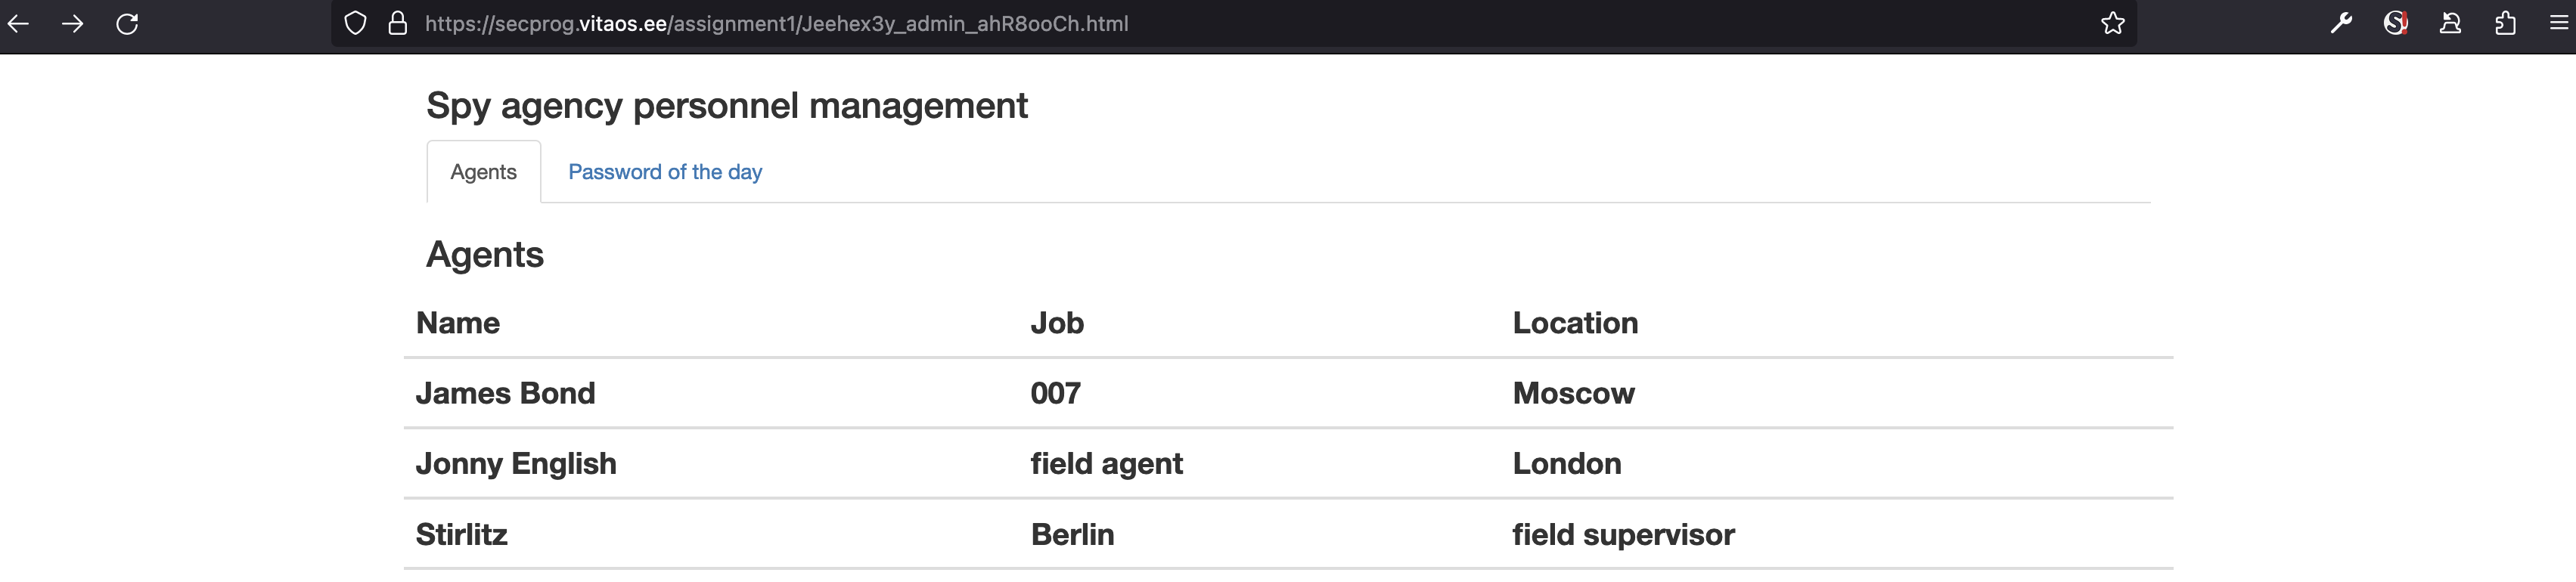
\includegraphics[width=\textwidth]{adminpanel}
  \caption{Admin panel view}
  \label{fig:adminpanel}
\end{figure}

\textbf{Recommendations.} Enforce server-side authenticated access control for
accessing the admin panel. That is, do not allow access for non authenticated
(logged-in) users. Additionally, do not allow all users to view the sensitive
details of spies and to view or set the password of the day---implement a
permission system.

\section*{Vulnerability 2}

\textbf{Risk level.} critical

An adversary can recover and/or bypass login credentials and gain illegitimate
access to the website without proper authorisation, and thereby access protected
and potentially sensitive internal resources.

\textbf{Risk.} Illegitimate access to the website's administrative panel without
proper authorisation, given an attacker access to protected and potentially
sensitive internal resources. It results in a breach of secrecy of data, which
is a privacy and national or even international risk (spy data).

The attack vectors are of a combination of client side authentication,
client-side credential storage, weak hashing, weak/known passwords. A
client-side JavaScript snippet validates input credentials against hardcoded
values. An attacker is able to determine the password that matches the expected
hash and/or modify password validation by replacing the JavaScript validation.

Potentially applicable OWASP categories are:
\begin{enumerate}
  \item \texttt{A02:2021} -- Cryptographic Failures%\footnote{\url{https://owasp.org/Top10/A02_2021-Cryptographic_Failures/}}
  \item \texttt{A07:2021} -- Identification and Authentication Failures%\footnote{\url{https://owasp.org/Top10/A07_2021-Identification_and_Authentication_Failures/}}
  \item \texttt{A01:2021} -- Broken Access Control%\footnote{\url{https://owasp.org/Top10/A01_2021-Broken_Access_Control/}}
  \item \texttt{A04:2021} -- Insecure Design%\footnote{\url{https://owasp.org/Top10/A04_2021-Insecure_Design/}}
\end{enumerate}

\textbf{Proof of Concept.}

\begin{enumerate}
  \item Navigate to\\
  \url{https://secprog.vitaos.ee/assignment1/Jeehex3y_admin_ahR8ooCh.html},
  \item View the page source in developer tools, or by downloading the webpage
  (\figref{fig:sourcecode}),
  \item Decode the base-64 encoded string ``\texttt{dmFyI\dots iKTs=}''
  (\figref{fig:b64decode}),
  \item Determine that the expected username is ``admin'',
  \item Use a reverse-hash lookup tool to look up,
\begin{center}
  \texttt{2ab96390c7dbe3439de74d0c9b0b1767}
\end{center}
  and determine that the expected password value is ``hunter2''\footnotemark,
\footnotetext{\url{https://md5.gromweb.com/?md5=2ab96390c7dbe3439de74d0c9b0b1767}}
  \item Log in with the credentials ``admin'' and ``hunter2''.
  \item Alternatively, paste the following in the browser's console for the
  webpage:
\begin{verbatim}
function doSmth(){
  var password=document.getElementById("password").value;
  var user=document.getElementById("user").value;
  ""==user && ""==password ?
    window.location.href="Jeehex3y_admin_ahR8ooCh.html" :
    alert("Wrong password or email");
}
document.getElementById("submit").addEventListener("click",doSmth,!1);
\end{verbatim}
  and then click on ``Login'', and ``OK'' on the pop-up, and then the
  redirection will happen regardless of empty credentials.
  (\figref{fig:jsattack})
\end{enumerate}

\begin{figure}
  \centering
  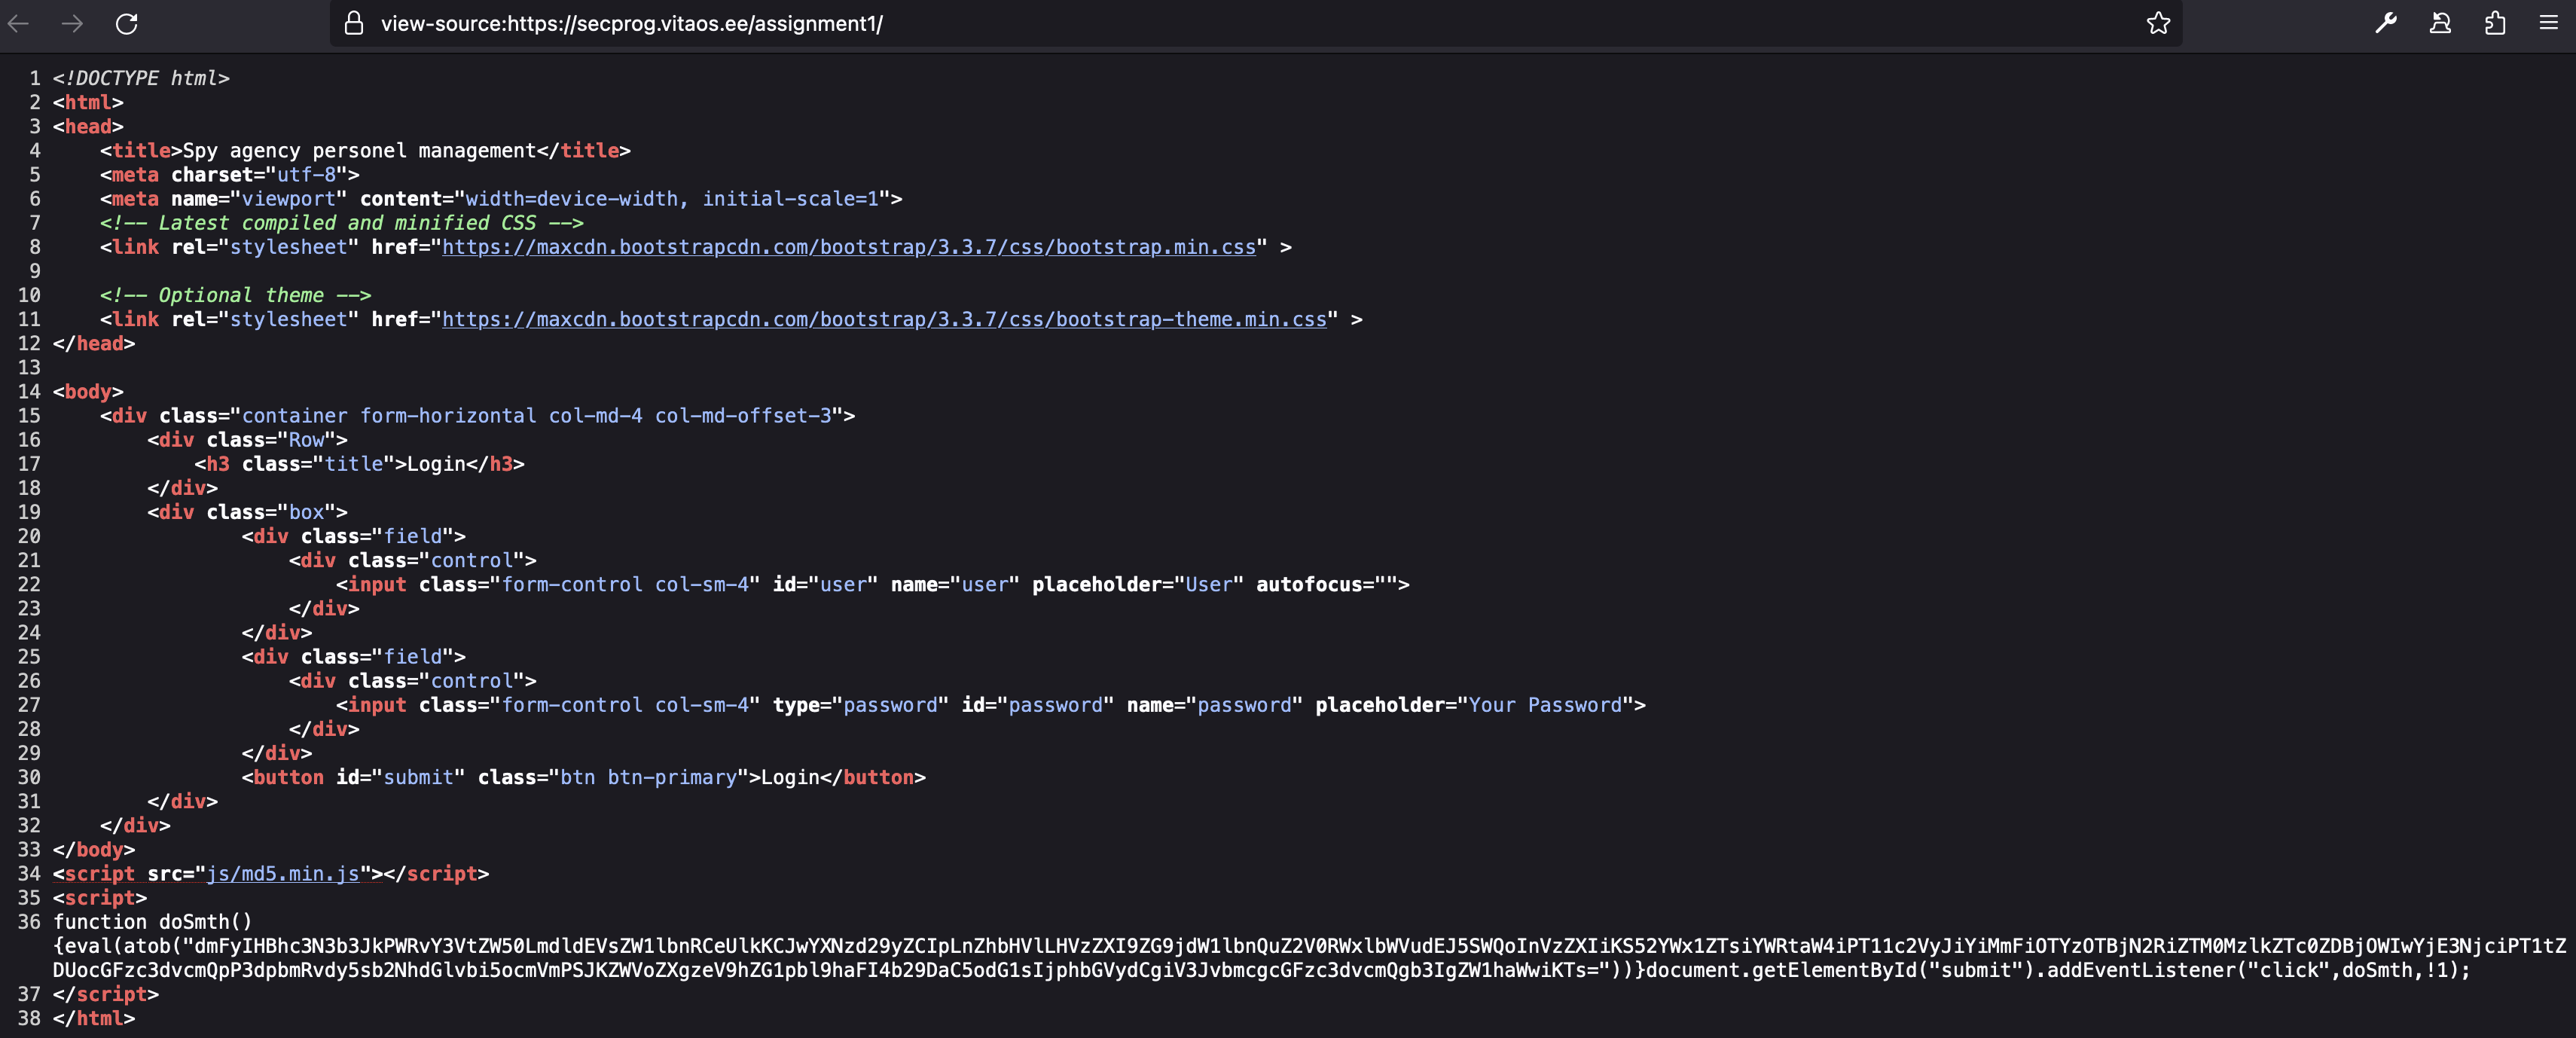
\includegraphics[width=\textwidth]{sourcecode}
  \caption{Website source}
  \label{fig:sourcecode}
\end{figure}

\begin{figure}
  \centering
  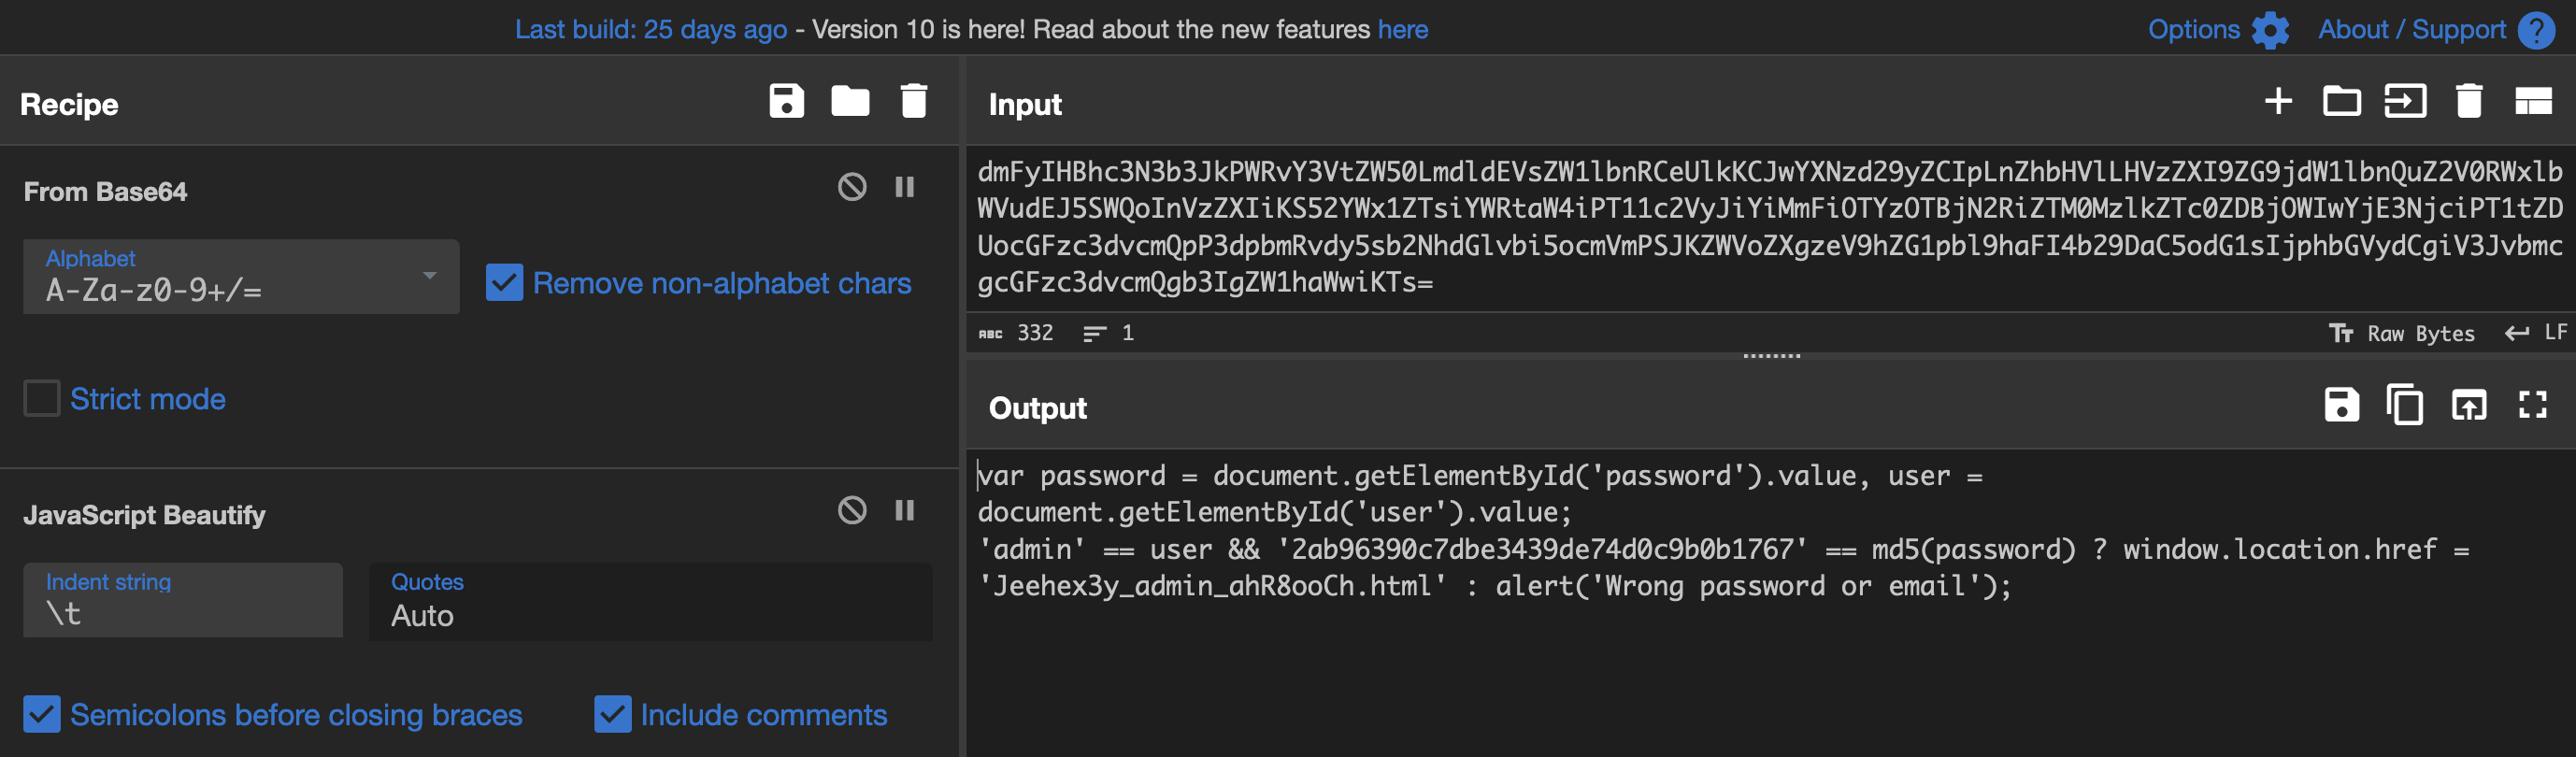
\includegraphics[width=\textwidth]{b64decode}
  \caption{Base64 decoding with CyberChef}
  \label{fig:b64decode}
\end{figure}

\begin{figure}
  \centering
  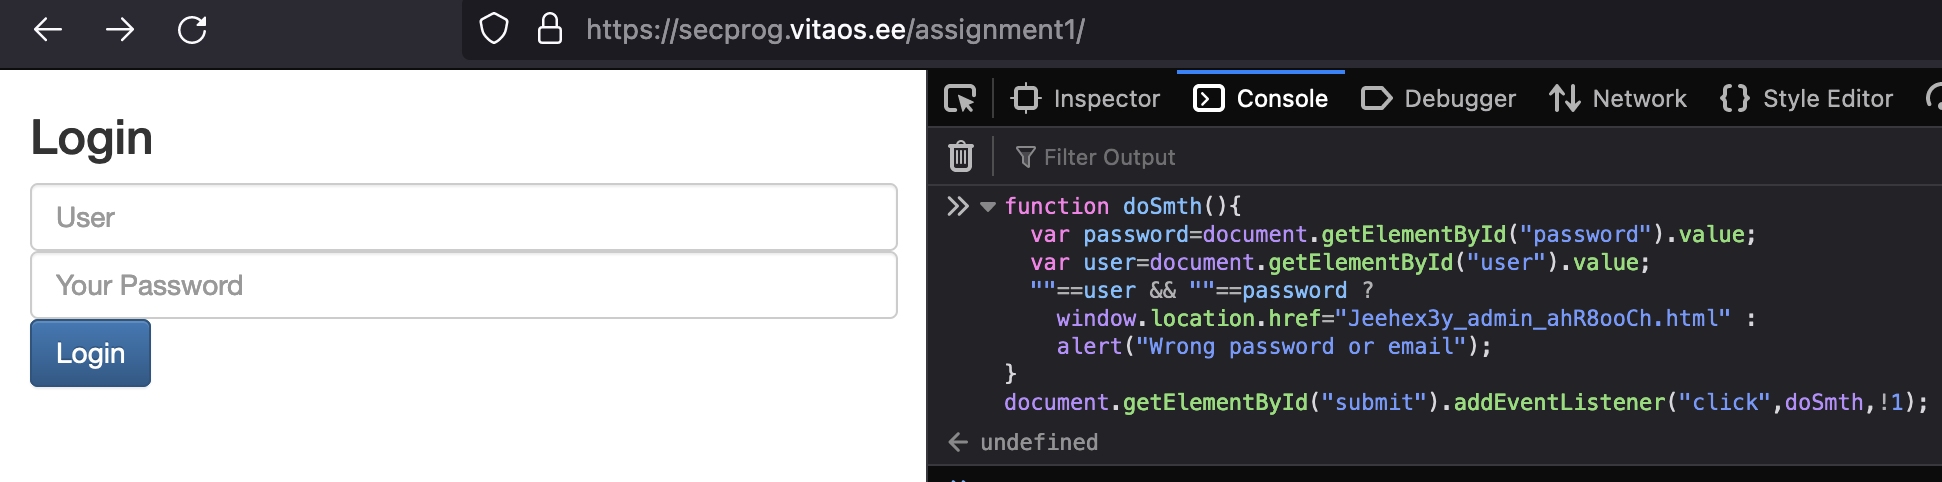
\includegraphics[width=\textwidth]{jsattack}
  \caption{JS function replacement}
  \label{fig:jsattack}
\end{figure}

\textbf{Recommendations.} Authenticate users on the server-side, and not on the
client side. Additionally, do not use weak hashing algorithms for password
storage, instead use specifically designed hash functions, such as those with
key stretching (e.g., scrypt, Argon2).

To protect password secrecy even more, use password salting for additional
protection against dictionary attacks, and enforce password minimum length and
complexity requirements, if feasible from a usability standpoint.

\section*{Vulnerability 3}

\textbf{Risk level.} moderate

The website allows insecure (non-encrypted) connections.

\textbf{Risk.} Credentials and data exchanged between client and server could
be sniffed by an adversary, therefore learning of private and potentially
sensitive information.

The attack vector is insecure web traffic, where encryption is not used to
protect data from an eavesdropper/sniffer.

Potentially applicable OWASP categories are:
\begin{enumerate}
  \item \texttt{A02:2021} -- Cryptographic Failures%\footnote{\url{https://owasp.org/Top10/A02_2021-Cryptographic_Failures/}}
\end{enumerate}

\textbf{Proof of Concept.}

\begin{enumerate}
  \item Navigate to\\
  \url{http://secprog.vitaos.ee/assignment1/Jeehex3y_admin_ahR8ooCh.html},
  \item Some browsers may force HTTPS redirect, so use \texttt{curl} to verify
  that there is no redirecting from HTTP. (\figref{fig:http})
\begin{verbatim}
curl -v -X OPTIONS http://secprog.vitaos.ee/assignment1/
\end{verbatim}
  Observe \texttt{HTTP/1.1 200 OK}, which shows that the resource is accessible
  over HTTP and there is no redirect.
\end{enumerate}

\textbf{Recommendations.} Enable and enforce HTTPS connections on the server.

\begin{figure}
  \centering
  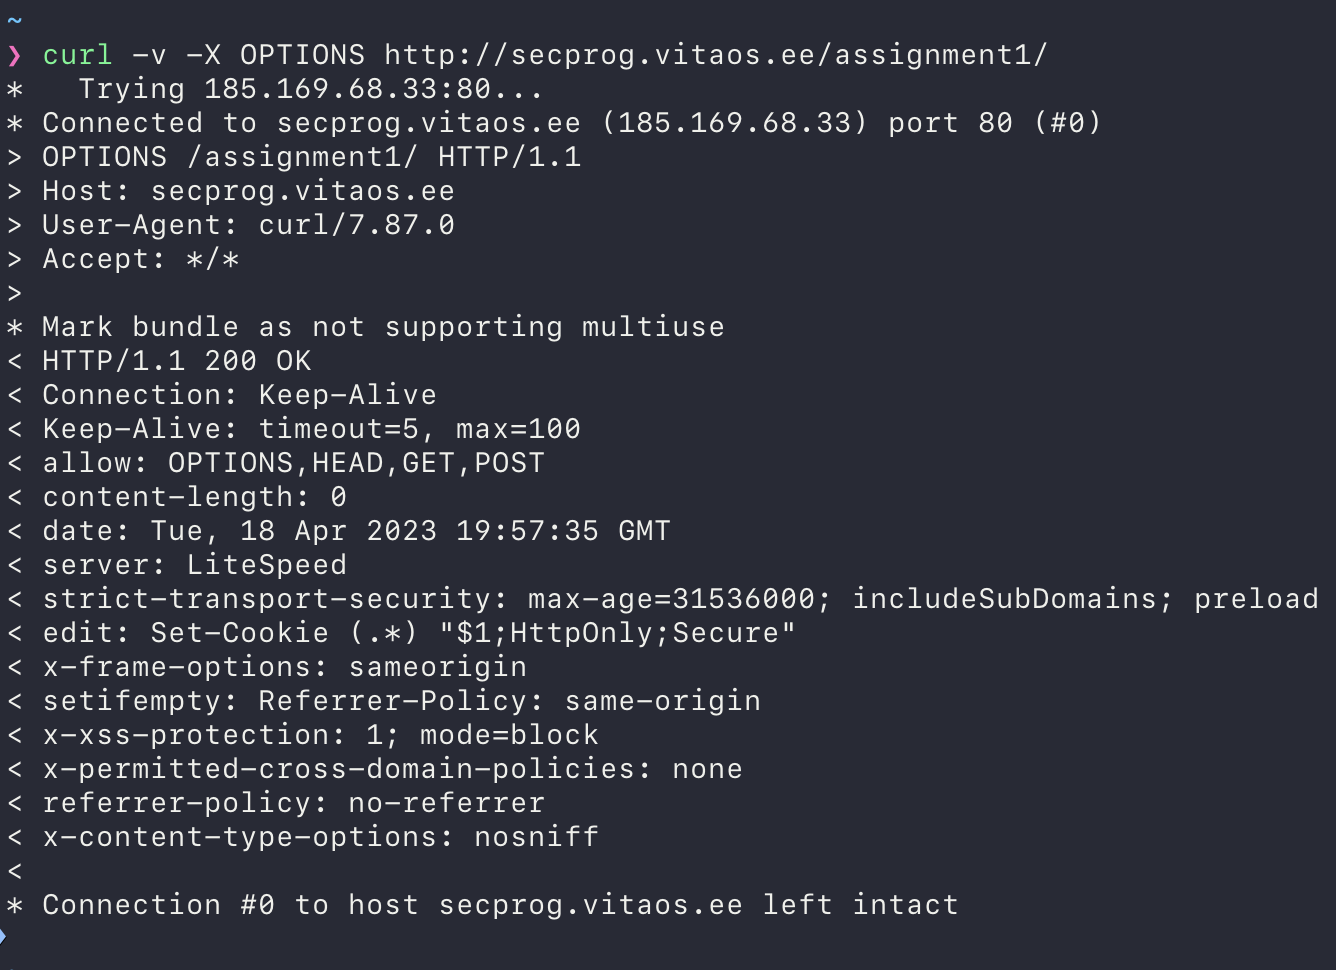
\includegraphics[width=\textwidth]{http}
  \caption{No redirect for HTTP}
  \label{fig:http}
\end{figure}

\section*{Addendum}

Log in credentials:
\begin{itemize}
  \item username: \texttt{admin}
  \item password: \texttt{hunter2}
\end{itemize}

Password of the day: \texttt{Dai1chaN}

Agents:

\begin{center}
\begin{tabular}{ | l | l | l | }
  \hline
  Name & Job & Location\\
  \hline
  \hline
  James Bond & 007 & Moscow\\
  Jonny English & field agent & London\\
  Stirlitz & Berlin & field supervisor\\
  \hline
\end{tabular}
\end{center}

\end{document}
